%%%%%%%%%%%%%%%%%%%%%%%%%%%%%%%%%%%%%%%%%%%%%%%%%%%%%%%%%%%%%%%%%%%%%%%%%%%%%%%%
%2345678901234567890123456789012345678901234567890123456789012345678901234567890
%        1         2         3         4         5         6         7         8

\documentclass[letterpaper, 10 pt, conference]{ieeeconf}  % Comment this line out
                                                          % if you need a4paper
%\documentclass[a4paper, 10pt, conference]{ieeeconf}      % Use this line for a4
                                                          % paper

\IEEEoverridecommandlockouts                              % This command is only
                                                          % needed if you want to
                                                          % use the \thanks command
\overrideIEEEmargins

% Packages
\usepackage{amsmath,amssymb}
\let\proof\relax
\let\endproof\relax
\usepackage{amsthm}
\usepackage{graphicx}
\usepackage{booktabs}
\usepackage[hypertexnames=false]{hyperref}
\let\labelindent\relax
\usepackage{enumitem}
\usepackage{listings}
\usepackage{xcolor}
\usepackage{tikz}
\usepackage{algorithm}
\usepackage{algpseudocode}
\usetikzlibrary{automata, positioning, arrows.meta}

% Theorem environments
\newtheorem{theorem}{Theorem}[section]
\newtheorem{lemma}[theorem]{Lemma}
\newtheorem{corollary}[theorem]{Corollary}
\newtheorem{definition}[theorem]{Definition}

% Notation
\newcommand{\EBel}[1]{\ensuremath{\Delta #1}} % Explicit Belief
\newcommand{\IBel}[1]{\ensuremath{\Box #1}}   % Implicit Belief
\newcommand{\CG}{\ensuremath{\mathit{CG}}}    % Common Ground

% Code listing style
\lstset{
    language=Python,
    basicstyle=\small\ttfamily,
    keywordstyle=\color{blue!70!black}\bfseries,
    commentstyle=\color{green!50!black}\itshape,
    stringstyle=\color{red!60!black},
    showstringspaces=false,
    numbers=left,
    numberstyle=\tiny\color{gray},
    breaklines=true,
    frame=single,
    framesep=3pt,
    backgroundcolor=\color{gray!5},
    tabsize=4,
}

\title{\LARGE \bf
Epistemic Reinforcement Learning for the Chop Cup:\\
SAT-Based Belief Reasoning with Reward Machines
}

\author{}


\begin{document}



\maketitle
\thispagestyle{empty}
\pagestyle{empty}


%%%%%%%%%%%%%%%%%%%%%%%%%%%%%%%%%%%%%%%%%%%%%%%%%%%%%%%%%%%%%%%%%%%%%%%%%%%%%%%%
\begin{abstract}

This paper presents a formal implementation of epistemic reinforcement learning for the Chop Cup, a canonical magic trick requiring systematic manipulation of an observer's belief state. We model the domain as a belief-base partially observable Markov decision process (BB-POMDP) where an agent (the Magician) must induce false beliefs in an observer through sequences of deceptive actions. Explicit beliefs ($\Delta$) are maintained as state fluents with update semantics derived from the formal action specification. Implicit beliefs ($\Box$) are computed via SAT-based entailment operating over the observer's knowledge base. We augment the MDP with a reward machine encoding the temporal structure of the deception protocol through condition-based transitions evaluated on the joint physical-epistemic state. Learning is performed using BEQRM (Belief-Enhanced Q-Learning for Reward Machines), which decomposes the value function over reward machine states to enable efficient credit assignment under sparse rewards.

\end{abstract}


%%%%%%%%%%%%%%%%%%%%%%%%%%%%%%%%%%%%%%%%%%%%%%%%%%%%%%%%%%%%%%%%%%%%%%%%%%%%%%%%
\section{INTRODUCTION}

Standard reinforcement learning optimizes for physical goals: reaching a target, maximizing score, or controlling a system. In contrast, \textbf{epistemic RL} optimizes for \emph{mental state manipulation}: the agent's goal is to change what another agent \emph{believes}, not merely what is physically true.

The Chop Cup magic trick provides an ideal testbed for this paradigm. A magician must:
\begin{enumerate}
    \item Navigate two parallel realities: \textbf{Physical Reality} (where objects actually are) and the \textbf{Observer's Belief} (where the Observer thinks objects are).
    \item Reach a state of \textbf{False Belief}: the Observer logically concludes $\phi$, but reality is $\neg\phi$.
    \item Exploit \emph{logical deduction} rather than simple observation gaps. The Observer reasons from background knowledge and direct observations using propositional logic.
\end{enumerate}

This report describes the design, implementation, and evaluation of a complete Python system that realizes this paradigm. The system is built upon the BB-POMDP framework~\cite{engesser2025} and the \texttt{epirl} Rust codebase\footnote{\url{https://github.com/tengesser/epirl}}, re-implemented in Python for accessibility and extensibility. Every action effect faithfully mirrors the \texttt{magic\_cup.json} specification, verified by a comprehensive audit against the JSON formulas.

%%%%%%%%%%%%%%%%%%%%%%%%%%%%%%%%%%%%%%%%%%%%%%%%%%%%%%%%%%%%%%%%%%%%%%%%%%%%%%%%
\section{THE CHOP CUP TRICK}

We model the classic Chop Cup with \textbf{1 cup and 2 balls}:
\begin{itemize}
    \item \textbf{Magnetic Ball}: Permanently stuck inside the cup via a magnet. Hidden from the Observer.
    \item \textbf{Regular Ball}: The visible ball that can be palmed, placed under the cup, or shown on the table.
\end{itemize}

The trick works because the Observer does not know about the magnetic ball. When the magician secretly palms the regular ball but the Observer sees it ``go under the cup,'' the Observer \emph{logically deduces} the ball must be under the cup. When the cup is lifted, the magnetic ball appears, creating the illusion that the ball magically reappeared.

\textbf{Deception Condition (Success):}
\[
    \IBel{\phi} \;\land\; \neg\phi \qquad \text{(Observer concludes $\phi$, but reality is $\neg\phi$)}
\]

For the Chop Cup, success means:
\[
    \IBel{\text{reg\_under}} \;\land\; \text{reg\_hand}
\]
The Observer believes the regular ball is under the cup, but it is actually in the magician's hand.

%%%%%%%%%%%%%%%%%%%%%%%%%%%%%%%%%%%%%%%%%%%%%%%%%%%%%%%%%%%%%%%%%%%%%%%%%%%%%%%%
\section{TECHNICAL FRAMEWORK}

\subsection{State Representation}

The environment state is a \textbf{factored set of boolean fluents}, partitioned into two groups.
\textbf{Physical fluents} represent the actual world state: \texttt{mag\_stuck} (magnetic ball stuck in cup), \texttt{mag\_visible} (magnetic ball visible when cup lifted), \texttt{reg\_under}, \texttt{reg\_table}, \texttt{reg\_hand} (regular ball location), and \texttt{cup\_down} (cup is covering its contents).
\textbf{Epistemic fluents} ($\Delta$) represent the Observer's explicit beliefs: $\EBel{\text{reg\_under}}$, $\EBel{\neg\text{reg\_under}}$, $\EBel{\text{reg\_table}}$, $\EBel{\neg\text{reg\_table}}$, $\EBel{\text{reg\_hand}}$, $\EBel{\neg\text{reg\_hand}}$, $\EBel{\text{lime\_cup}}$, $\EBel{\neg\text{lime\_cup}}$.

Implicit beliefs ($\IBel{\cdot}$) are \emph{not} stored as fluents. They are computed on-demand by the SAT solver.

\subsection{Epistemic Logic Engine}

The Observer's reasoning is modeled using three components:

\subsubsection{Common Ground (\texorpdfstring{$\CG$}{CG})}
The Common Ground represents background knowledge that the Observer uses to reason about the world. Critically, the Observer believes there is only \emph{one} ball (they have no idea a hidden magnetic ball exists inside the cup). When the Observer deduces where the ball is, they apply a simple commonsense rule: the ball must be in \emph{exactly one} location. This is encoded as an \textbf{exclusive-or} constraint:
\[
    \CG:\; \text{reg\_under} \oplus \text{reg\_table} \oplus \text{reg\_hand}
\]
\vspace{-1ex}\noindent(i.e., exactly one location is true).
From the Observer's perspective, this simply says ``the ball is either under the cup, on the table, or in the magician's hand, but not in multiple places at once.'' The fluent names use the prefix \texttt{reg\_} (for ``regular ball'') in our implementation, but the Observer does not make this distinction; to them, these describe where ``the ball'' is.

Logically, the constraint means: the ball must be \emph{somewhere} (at least one location is true), but cannot be in \emph{multiple places} simultaneously (at most one location is true). In propositional logic, where $x_i, x_j \in \{\text{reg\_under}, \text{reg\_table}, \text{reg\_hand}\}$:
\[
    (\text{reg\_under} \lor \text{reg\_table} \lor \text{reg\_hand}) 
    \;\land\; 
    \bigwedge_{i < j} (\neg x_i \lor \neg x_j)
\]
The second part says ``for every pair of locations, they cannot both be true simultaneously.'' This gives us three clauses: $(\neg\text{reg\_under} \lor \neg\text{reg\_table})$, $(\neg\text{reg\_under} \lor \neg\text{reg\_hand})$, and $(\neg\text{reg\_table} \lor \neg\text{reg\_hand})$.

This constraint is what enables the deception: when the Observer deduces that the ball is \emph{not} on the table and \emph{not} in the hand, the Common Ground forces them to conclude it must be under the cup. The Observer's reasoning is perfectly valid given their knowledge, but their conclusion is wrong because they are unaware of the magnetic ball. The false belief arises from missing information, not from a logical error.

\subsubsection{Explicit Beliefs (\texorpdfstring{$\EBel{\phi}$}{Delta phi})}
Direct observations stored as fluents. Actions generate belief updates through \textbf{belief transfer effects} (matching JSON notation $\triangle p := f$).
For \texttt{palm\_ball}: $\EBel{\text{reg\_under}} \gets \EBel{\text{reg\_table}}$ (the key transfer).
For \texttt{lift\_cup}: $\EBel{\neg\text{reg\_under}} \gets \top$, $\EBel{\text{reg\_table}} \gets \EBel{\text{reg\_table}} \lor \text{reg\_under}$.
For \texttt{place\_cup}: $\EBel{\text{reg\_under}} \gets \EBel{\text{reg\_table}}$.
For \texttt{reveal\_hand}: $\EBel{\text{reg\_hand}} \gets \text{reg\_hand}$.

\subsubsection{Implicit Beliefs (\texorpdfstring{$\IBel{\phi}$}{Box phi}) via SAT Entailment}
The SAT solver derives what the Observer \emph{must} believe:
\[
    \IBel{\phi} \quad \iff \quad \underbrace{\CG \;\land\; \bigwedge_i \EBel{\psi_i}}_{KB} \;\land\; \neg\phi \quad \text{is UNSAT}
\]

We implement a lightweight SAT solver sufficient for the small propositional theories in the Chop Cup domain.

\begin{algorithm}[h]
\caption{Implicit Belief Query via SAT Entailment}
\begin{algorithmic}[1]
\Function{ImplicitBelief}{$\phi$, $\text{positive}$, $\CG$, $\Delta$}
    \State $KB \gets \CG.\text{clauses} \cup \Delta.\text{clauses}$
    \If{positive}
        \State $KB \gets KB \cup \{\{\neg\phi\}\}$ \Comment{Query: $KB \land \neg\phi$}
    \Else
        \State $KB \gets KB \cup \{\{\phi\}\}$ \Comment{Query: $KB \land \phi$}
    \EndIf
    \State \Return $\neg\text{SAT}(KB)$ \Comment{$\IBel{\phi}$ iff UNSAT}
\EndFunction
\end{algorithmic}
\end{algorithm}

\subsubsection*{Key Example: The Deception via Belief Transfer}
The \texttt{palm\_ball} action is the core deceptive act. Its JSON effects include the critical \textbf{belief transfer}:
\[
    \triangle\text{reg\_under} := \triangle\text{reg\_table}
\]
Before the palm, $\EBel{\text{reg\_table}} = \top$ (observer sees ball on table). After the palm:
\begin{align*}
    \EBel{\text{reg\_under}} &= \top \quad \text{(transferred from } \EBel{\text{reg\_table}}\text{)} \\
    \EBel{\neg\text{reg\_table}} &= \top \quad \text{(ball ``left'' the table)} \\
    \EBel{\neg\text{reg\_hand}} &= \top \quad \text{(observer doesn't detect ball in hand)}
\end{align*}
The SAT solver then \textbf{confirms} the explicit belief: $\CG \land \EBel{\neg\text{table}} \land \EBel{\neg\text{hand}} \land \neg\text{reg\_under}$ is UNSAT, so $\IBel{\text{reg\_under}} = \top$. The Observer is now fully deceived: they believe the ball is under the cup, but it is actually in the magician's hand.

\addtolength{\textheight}{-3cm}   % This command serves to balance the column lengths
                                  % on the last page of the document manually.

%%%%%%%%%%%%%%%%%%%%%%%%%%%%%%%%%%%%%%%%%%%%%%%%%%%%%%%%%%%%%%%%%%%%%%%%%%%%%%%%
\section{REWARD MACHINE}

A \textbf{Reward Machine} (RM)~\cite{icarte2018} is a finite automaton that tracks progress through the magic trick, providing structured rewards for achieving deception milestones. Our RM uses \textbf{condition-based transitions}: after each action modifies the environment state, the RM evaluates epistemic/propositional conditions on the resulting state to determine transitions.

\subsection{RM States}

The RM has 6 states in total (5 effective without the lime finale):

\begin{center}
\begin{tabular}{cll}
\toprule
\textbf{State} & \textbf{Name} & \textbf{Meaning} \\
\midrule
$u_0$ & Setup & Initial state. Ball on table. \\
$u_1$ & Covered & $\EBel{\text{reg\_under}}$. \\
$u_2$ & Pocket & $\IBel{\text{reg\_hand}}$. \\
$u_3$ & Appear & \texttt{ball\_visible}. \\
$u_4$ & Lime Loaded & $\IBel{\neg\text{lime\_cup}}$. \\
$u_T$ & Milestone & Lime revealed; loops. \\
\bottomrule
\end{tabular}
\end{center}

State $u_4$ is only active when \texttt{enable\_limes = True}. In the base ball-only trick, the effective RM has 5 states: $\{u_0, u_1, u_2, u_3, u_T\}$. There is no terminal RM state; episodes end only when the step limit is reached. From $u_T$, the agent can loop back to $u_4$ to load additional limes.

\subsection{RM Automaton Diagram}

\begin{center}
\resizebox{\columnwidth}{!}{%
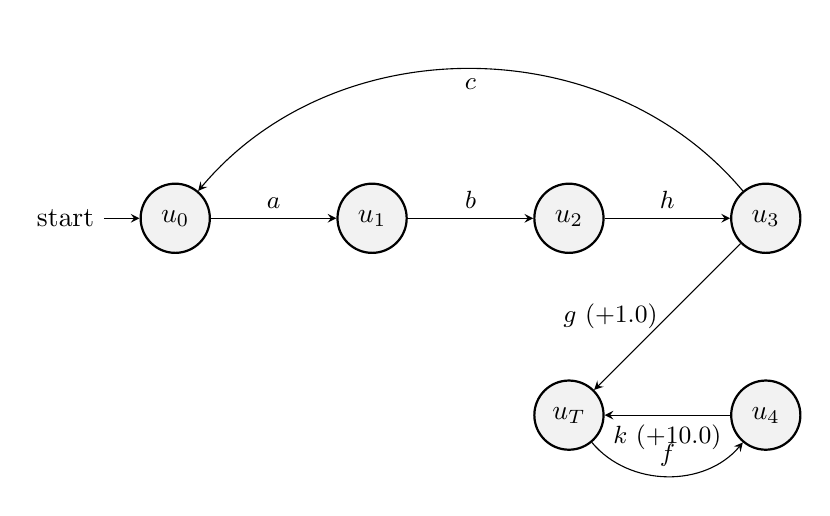
\begin{tikzpicture}[->, >=stealth, node distance=2.5cm, every state/.style={thick, fill=gray!10}]
% Standard Ball Cycle
\node[state, initial] (u0) {$u_0$};
\node[state, right of=u0] (u1) {$u_1$};
\node[state, right of=u1] (u2) {$u_2$};
\node[state, right of=u2] (u3) {$u_3$};

% Lime Finale Branch
\node[state, below of=u3] (u4) {$u_4$};
\node[state, left of=u4] (uT) {$u_T$};

% Ball Transitions
\path
    (u0) edge node[above] {\small $a$} (u1)
    (u1) edge node[above] {\small $b$} (u2)
    (u2) edge node[above] {\small $h$} (u3)
    (u3) edge[bend right=50] node[below] {\small $c$} (u0)
    (u3) edge node[left] {\small $g$ (+1.0)} (uT);

% Lime Transitions
\path
    (u4) edge node[below] {\small $k$ (+10.0)} (uT)
    (uT) edge[bend right=50] node[above] {\small $f$} (u4);
\end{tikzpicture}}
\end{center}

All transitions are solid; the lime finale ($u_4$ to $u_T$) is fully active when \texttt{enable\_limes = True}. Note that $u_T$ is \emph{not} a terminal state: there is a loop from $u_T$ back to $u_4$ allowing the agent to load additional limes. Episodes end only when the step limit is reached.

\subsection{Condition-Based Transitions}

Each RM transition has a propositional or epistemic \textbf{condition} evaluated against the environment state \emph{after} the action's effects are applied. This contrasts with action-triggered RMs where transitions are encoded inside action effects.

\begin{center}
\resizebox{\columnwidth}{!}{%
\begin{tabular}{cllp{2.5cm}}
\toprule
\textbf{Lbl} & \textbf{Trans.} & \textbf{Condition} & \textbf{Description} \\
\midrule
$a$ & $u_0 \!\to\! u_1$ & $\EBel{\text{reg\_under}}$ & Sees ball ``under'' \\
$b$ & $u_1 \!\to\! u_2$ & $\IBel{\text{reg\_hand}}$ & Infers ball in hand \\
$h$ & $u_2 \!\to\! u_3$ & \texttt{ball\_visible} & Ball appears \\
$c$ & $u_3 \!\to\! u_0$ & \texttt{cup\_down} & Reset cycle \\
$g$ & $u_3 \!\to\! u_T$ & \texttt{ball\_vis.}$\land$$\neg$\texttt{lime\_v.} & \textbf{Deceived! (+1)} \\
\midrule
$k$ & $u_4 \!\to\! u_T$ & \texttt{lime\_visible} & \textbf{Lime! (+10)} \\
$f$ & $u_T \!\to\! u_4$ & $\IBel{\neg\text{lime\_cup}}$ & Loop for limes \\
\bottomrule
\end{tabular}}
\end{center}

Note that transition $b$ uses an \textbf{implicit belief} ($\IBel{\text{reg\_hand}}$), computed by the SAT solver. This is the only RM transition that requires epistemic reasoning rather than simple fluent checks.

\subsection{Reward Structure}

The \textbf{main reward} is $+1.0$ on transition $g$ ($u_3 \to u_T$) and $+10.0$ on transition $k$ ($u_4 \to u_T$). These represent successful deception milestones. The RM has no terminal state; episodes end only when the step limit (\texttt{max\_steps}) is reached.

\subsection{State Space and Action Space}

\subsubsection{Action Space}
The agent has 4 base actions (plus 1 extended action when limes are enabled):

\begin{center}
\resizebox{\columnwidth}{!}{%
\begin{tabular}{lll}
\toprule
\textbf{Action} & \textbf{Key Effect} & \textbf{Epistemic Effect} \\
\midrule
\texttt{lift\_cup} & Reveals contents & $\EBel{\neg\text{reg\_under}} \!\gets\! \top$ \\
\texttt{place\_cup} & Covers contents & $\EBel{\text{reg\_under}} \!\gets\! \EBel{\text{reg\_table}}$ \\
\texttt{palm\_ball} & Ball $\to$ hand & $\EBel{\text{reg\_under}} \!\gets\! \EBel{\text{reg\_table}}$ \\
\texttt{reveal\_hand} & Show hand & $\EBel{\text{reg\_hand}} \!\gets\! \text{reg\_hand}$ \\
\midrule
\texttt{load\_lime} & Hide lime & (no belief change) \\
\bottomrule
\end{tabular}}
\end{center}

\subsubsection{State Space}

The RL observation is a cross-product of environmental state and RM state:

\begin{enumerate}
    \item \textbf{Physical state} (10 features): \texttt{mag\_stuck}, \texttt{mag\_visible}, \texttt{reg\_under}, \texttt{reg\_table}, \texttt{reg\_hand}, \texttt{cup\_down}, \texttt{ball\_visible}, \texttt{lime\_cup}, \texttt{lime\_visible}, \texttt{lime\_count}.
    \item \textbf{Belief state} (8 features): $\EBel{\text{reg\_under}}$, $\EBel{\neg\text{reg\_under}}$, $\EBel{\text{reg\_table}}$, $\EBel{\neg\text{reg\_table}}$, $\EBel{\text{reg\_hand}}$, $\EBel{\neg\text{reg\_hand}}$, $\EBel{\text{lime\_cup}}$, $\EBel{\neg\text{lime\_cup}}$.
    \item \textbf{RM state}: One of $\{u_0, u_1, u_2, u_3, u_4, u_T\}$ (6 states).
\end{enumerate}

%%%%%%%%%%%%%%%%%%%%%%%%%%%%%%%%%%%%%%%%%%%%%%%%%%%%%%%%%%%%%%%%%%%%%%%%%%%%%%%%
\section{CONVERGENCE OF EPISTEMIC QRM}
\label{sec:convergence}

A natural question arises when augmenting the QRM state space with epistemic (belief) features: does Q-learning still converge to an optimal policy?
In this section we provide a formal proof that it does, by showing that the epistemic QRM formulation reduces to standard Q-learning on a well-defined MDP.

\subsection{Epistemic Cross-Product MDP}

\begin{definition}[Epistemic MDP with Reward Machine]
\label{def:epi-mdp}
Let $M_{\mathrm{env}} = (S_{\mathrm{env}},\, A,\, T,\, \gamma)$ be a finite environment MDP whose state decomposes as
\[
    s = (s_{\mathrm{phys}},\; s_{\mathrm{bel}}) \;\in\; S_{\mathrm{env}},
\]
where $s_{\mathrm{phys}} \in \{0,1\}^{n_p}$ is a vector of physical fluents and $s_{\mathrm{bel}} \in \{0,1\}^{n_b}$ is a vector of explicit-belief fluents ($\EBel{\cdot}$).  The action set $A$ is finite, and the transition function $T : S_{\mathrm{env}} \times A \to S_{\mathrm{env}}$ is deterministic.

A \emph{reward machine} is a tuple $\mathcal{R} = (U,\, u_0,\, \delta_u,\, \delta_r)$, where $U$ is a finite set of RM states, $u_0 \in U$ is the initial state, $\delta_u : U \times 2^{\mathcal{P}} \to U$ is a deterministic transition function conditioned on a set of propositional/epistemic labels $L(s) \subseteq \mathcal{P}$ evaluated on the environment state, and $\delta_r : U \times U \to \mathbb{R}$ assigns a bounded reward to each RM transition.
\end{definition}

\begin{definition}[Augmented (Cross-Product) MDP]
\label{def:cross-product}
Define the augmented MDP
\[
    \tilde{M} \;=\; \bigl(\tilde{S},\; A,\; \tilde{T},\; \tilde{R},\; \gamma\bigr)
\]
with the following components.
The \textbf{augmented state space} is $\tilde{S} = S_{\mathrm{env}} \times U$, where each state is a triple $\tilde{s} = (s_{\mathrm{phys}},\, s_{\mathrm{bel}},\, u)$.
The \textbf{transition function} is
\[
    \tilde{T}\!\bigl((s,u),a,(s',u')\bigr) \!=\!
    \begin{cases}
        T(s,a,s') & \text{if } u' = \delta_u(u,L(s')), \\
        0 & \text{otherwise}.
    \end{cases}
\]
The \textbf{reward function} is
$\tilde{R}\bigl((s, u),\, a,\, (s', u')\bigr) = \delta_r(u, u')$.
\end{definition}

\begin{lemma}[Markov property]
\label{lem:markov}
In the augmented MDP $\tilde{M}$, the reward $\tilde{R}$ and transition $\tilde{T}$ depend only on the current augmented state $(s, u)$ and action $a$, not on the history of previously visited states.
\end{lemma}

\begin{proof}
By construction of Definition~\ref{def:cross-product}:
\begin{enumerate}
    \item $T(s,a,s')$ is a function of $(s, a)$ alone, since the environment transition function is deterministic.
    \item $L(s')$ is a function of the resulting environment state $s'$ only: explicit beliefs $\EBel{\phi}$ are fluents within $s$, and implicit beliefs $\IBel{\phi}$ are computed by SAT entailment over the Common Ground $\CG$ and the explicit beliefs in $s'$.  Critically, $\CG$ is \emph{fixed} (it does not change across time steps), so $\IBel{\phi}$ is a deterministic function of $s'$.
    \item $\delta_u(u, L(s'))$ is a deterministic function of $(u, s')$.
    \item $\delta_r(u, u')$ depends only on the RM transition $(u, u')$.
\end{enumerate}
Therefore, all components of the augmented transition and reward functions are determined by $(s, u, a)$ without reference to history. The augmented MDP satisfies the Markov property. \qed
\end{proof}

\noindent\textbf{Remark.}
The key insight is that \emph{implicit beliefs do not introduce history-dependence}.  Although $\IBel{\phi}$ is computed via SAT entailment ($\CG \land \bigwedge_i \EBel{\psi_i} \land \neg\phi$ is UNSAT?), the inputs to this computation, the Common Ground and the explicit beliefs, are fully contained in the current state $s$.  Furthermore, explicit beliefs are updated by deterministic action effects (belief transfer semantics $\EBel{p} \gets f(s)$), so they, too, are determined by $(s, a)$ alone.

\subsection{Q-Learning on the Augmented MDP}

Our QRM agent maintains a Q-table indexed by the augmented state:
\[
    Q : \tilde{S} \times A \to \mathbb{R}, \qquad
    Q\bigl[(s_{\mathrm{phys}},\, s_{\mathrm{bel}},\, u),\; a\bigr].
\]
On each transition $(s, u) \xrightarrow{a} (s', u')$ with reward $r = \delta_r(u, u')$, the update rule is standard tabular Q-learning:
\begin{multline}
\label{eq:q-update}
Q\bigl[(s,u),a\bigr] \leftarrow Q\bigl[(s,u),a\bigr] \\
    + \alpha\bigl[r + \gamma\max_{a'} Q[(s',u'),a'] - Q[(s,u),a]\bigr].
\end{multline}

\begin{theorem}[Convergence of Epistemic QRM]
\label{thm:convergence}
Under the following conditions:
\begin{enumerate}[label=(\roman*)]
    \item Every augmented state action pair $\bigl((s, u),\, a\bigr)$ is visited infinitely often.
    \item The learning rate sequence $\{\alpha_t\}$ satisfies the Robbins Monro conditions:
    \[
        \sum_{t=0}^{\infty} \alpha_t = \infty, \qquad \sum_{t=0}^{\infty} \alpha_t^2 < \infty.
    \]
    \item Rewards are bounded: $|\delta_r(u, u')| \leq R_{\max}$ for all $(u, u') \in U \times U$.
\end{enumerate}
Then the Q-values converge to the optimal Q-function with probability~1:
\[
    Q[(s,u),a] \xrightarrow{\;a.s.\;} Q^*[(s,u),a]
    \;\;\forall (s,u) \!\in\! \tilde{S},\, a \!\in\! A.
\]
Consequently, the greedy policy $\pi^*(s, u) = \arg\max_a Q^*\bigl[(s, u),\, a\bigr]$ is optimal in~$\tilde{M}$.
\end{theorem}

\begin{proof}
By Lemma~\ref{lem:markov}, $\tilde{M}$ is a well-defined MDP.  We verify the preconditions of the Watkins and Dayan convergence theorem.
First, the \emph{finite state space} condition holds: $|\tilde{S}| = |S_{\mathrm{env}}| \times |U| < \infty$, since both $S_{\mathrm{env}}$ (a product of finitely many boolean fluents) and $U$ are finite.
Second, the \emph{finite action space} condition holds: $|A| < \infty$ by assumption.
Third, \emph{bounded rewards} are guaranteed by condition~(iii), i.e.\ $|\delta_r(u,u')| \leq R_{\max}$ for all $(u, u')$.
Fourth, \emph{Markov transitions} are established by Lemma~\ref{lem:markov}.
The update rule~\eqref{eq:q-update} is precisely the tabular Q-learning algorithm of Watkins~\cite{watkins1992} applied to $\tilde{M}$.  Under conditions (i) to (iii), the convergence theorem of Watkins and Dayan~\cite{watkins1992} (see also Tsitsiklis~\cite{tsitsiklis1994} and Jaakkola et al.~\cite{jaakkola1994}) guarantees that $Q_t \to Q^*$ with probability~1.

The essential observation is that the belief fluents ($s_{\mathrm{bel}}$) and the RM state ($u$) are merely additional \emph{components} of the augmented state vector.  From the perspective of Q-learning, there is no distinction between a ``physical'' state feature and an ``epistemic'' state feature: both are elements of the finite state space $\tilde{S}$ over which the algorithm maintains Q-values.  The epistemic features ensure that the Markov property holds (Lemma~\ref{lem:markov}), and the RM state ensures that the non-Markov temporal reward structure becomes Markov.  Together, they produce a standard finite MDP to which classical convergence results apply directly. \qed
\end{proof}

\subsection{Extension to PBRS}

Theorem~\ref{thm:convergence} extends naturally to the QRM+PBRS variant (Section~\ref{sec:pbrs}).
By the Ng, Harada, Russell theorem~\cite{ng1999}, defining a shaped reward
\[
    R'(\tilde{s},\, a,\, \tilde{s}') = R(\tilde{s},\, a,\, \tilde{s}') + \gamma\,\Phi(u') - \Phi(u)
\]
with potential $\Phi : U \to \mathbb{R}$ produces a new MDP $\tilde{M}'$ whose set of optimal policies is identical to that of $\tilde{M}$.  Since $\tilde{M}'$ is itself a standard MDP with bounded rewards, Q-learning on $\tilde{M}'$ also converges under the same conditions (i) to (iii), and the resulting optimal policy is optimal for the original (unshaped) problem.

\begin{corollary}
Under conditions (i) to (iii), Q-learning with PBRS on the epistemic augmented MDP converges to an optimal policy of the original MDP $\tilde{M}$ with probability~1.
\end{corollary}

%%%%%%%%%%%%%%%%%%%%%%%%%%%%%%%%%%%%%%%%%%%%%%%%%%%%%%%%%%%%%%%%%%%%%%%%%%%%%%%%
\section{POTENTIAL-BASED REWARD SHAPING (PBRS)}
\label{sec:pbrs}

Our Reward Machine provides clear milestones but assigns \emph{sparse} rewards: the agent receives $+1$ only upon completing the ball deception ($u_3 \!\to\! u_T$, transition~$g$) and $+10$ for each lime reveal ($u_4 \!\to\! u_T$, transition~$k$).
All intermediate transitions carry zero reward.
Early in training, random exploration rarely reaches these milestones, so Q-values remain near zero across most of the state space and gradients are uninformative.

\textbf{Potential-Based Reward Shaping (PBRS)}~\cite{ng1999} addresses this sparsity by adding a \emph{shaping bonus} to every transition:
\begin{gather}
\label{eq:shaping}
R'(s, a, s') = R(s, a, s') + F(s, s'),\notag\\
F(s, s') = \gamma\,\Phi(s') - \Phi(s),
\end{gather}
where $\Phi : \mathcal{S} \to \mathbb{R}$ is a bounded \emph{potential function} of the state.
The crucial property is that $F$ depends \emph{only} on the states, not on the action, and has the specific $\gamma\Phi(s') - \Phi(s)$ form.

\paragraph{Policy invariance theorem (Ng, Harada and Russell, 1999).}
Let $M$ be an MDP with reward $R$ and let $M'$ be the MDP with shaped reward $R'$ as defined in~\eqref{eq:shaping}.
Then \emph{every optimal policy of~$M'$ is also an optimal policy of~$M$}, and vice versa.

\begin{proof}[Proof sketch (telescoping argument).]
Consider any trajectory $s_0, a_0, s_1, a_1, \ldots, s_T$ and its discounted return under $R'$:
\begin{multline}
\label{eq:telescope1}
G' = \sum_{t=0}^{T} \gamma^t R'(s_t, a_t, s_{t+1})
     = \sum_{t=0}^{T} \gamma^t R(s_t, a_t, s_{t+1})\\
       + \sum_{t=0}^{T} \gamma^t\bigl[\gamma\Phi(s_{t+1}) - \Phi(s_t)\bigr].
\end{multline}
The shaping terms telescope:
\begin{equation}
\label{eq:telescope2}
\sum_{t=0}^{T} \gamma^t[\gamma\Phi(s_{t+1}) - \Phi(s_t)]
  = \gamma^{T+1}\Phi(s_{T+1}) - \Phi(s_0).
\end{equation}
Since $\Phi(s_0)$ is a constant for any fixed initial state, and $\gamma^{T+1}\Phi(s_{T+1})$ depends only on the terminal state (not on the intermediate policy choices), the ranking of policies under $G'$ is identical to their ranking under~$G = \sum_t \gamma^t R(s_t,a_t,s_{t+1})$.
Therefore $\pi^* = \arg\max_\pi \mathbb{E}[G] = \arg\max_\pi \mathbb{E}[G']$; the optimal policy is invariant.
\end{proof}

In other words, PBRS reshuffles \emph{when} reward is received along a trajectory but does not change the \emph{total} ordering of policies. The agent converges faster because informative signal appears earlier, but the policy it converges \emph{to} is unchanged.

\paragraph{Potential function design.}
In BEQRM the RL state is the cross-product $(s_{\mathrm{env}},\, u)$ of environment state and RM state.  Because the RM already encodes task progress, we define $\Phi$ solely over the RM component:
\begin{equation}
\label{eq:potential}
\Phi(u) =
\begin{cases}
0 & u = u_0 \;\text{(Setup)},\\
1 & u = u_1 \;\text{(Covered)},\\
2 & u = u_2 \;\text{(Pocket)},\\
3 & u = u_3 \;\text{(Appear)},\\
4 & u = u_4 \;\text{(Lime Loaded)},\\
5 & u = u_T \;\text{(Milestone)}.
\end{cases}
\end{equation}
The values increase monotonically along the RM's forward path $u_0 \!\to\! u_1 \!\to\! u_2 \!\to\! u_3 \!\to\! u_T$, with $u_4$ assigned an intermediate value between $u_3$ and $u_T$ because it lies in the lime sub-loop.
The specific magnitudes are not critical: any monotonically increasing assignment preserves the same optimal policy; only the convergence speed is affected.

\paragraph{Concrete shaped rewards.}
Substituting $\gamma = 0.9$ and the potentials from~\eqref{eq:potential} into~\eqref{eq:shaping} yields the following shaped rewards for each RM transition:

\begin{table}[ht]
\centering\small
\begin{tabular}{clcrr}
\toprule
\textbf{Label} & \textbf{Transition} & $R$ & \textbf{Shaping} $F$ & $R'$ \\
\midrule
$a$ & $u_0 \to u_1$ & $0$ & $+0.9$ & $+0.9$ \\
$b$ & $u_1 \to u_2$ & $0$ & $+0.8$ & $+0.8$ \\
$h$ & $u_2 \to u_3$ & $0$ & $+0.7$ & $+0.7$ \\
$g$ & $u_3 \to u_T$ & $+1$ & $+1.5$ & $+2.5$ \\
$c$ & $u_3 \to u_0$ & $0$ & $-3.0$ & $-3.0$ \\
$f$ & $u_T \to u_4$ & $0$ & $-1.4$ & $-1.4$ \\
$k$ & $u_4 \to u_T$ & $+10$ & $+0.5$ & $+10.5$ \\
--- & no transition & $0$ & $-0.1\,\Phi(u)$ & $\leq 0$ \\
\bottomrule
\end{tabular}
\caption{Original reward~$R$, shaping bonus $F = \gamma\Phi(u') - \Phi(u)$, and shaped reward~$R' = R + F$ for each RM transition ($\gamma = 0.9$).}
\label{tab:shaped_rewards}
\end{table}

The shaped reward landscape differs markedly from the original.
Transitions that advance through the RM (rows $a$ to $h$, $g$, $k$) now carry \emph{positive} intermediate credit, even when the original reward is zero.
Conversely, the reset transition~$c$ ($u_3 \to u_0$) receives a penalty of $-3.0$ and the lime-loading loop~$f$ ($u_T \to u_4$) receives $-1.4$, discouraging backward progress unless it leads to the large lime reward $k$.
Steps that cause no RM transition receive a small negative signal $-0.1\,\Phi(u)$, nudging the agent to make progress rather than stall.

\paragraph{Effect on learning.}
The practical consequence is \emph{faster convergence}, not a different policy.
Without shaping, the agent must discover the sparse $+1$ at $u_3 \to u_T$ through random exploration before any useful Q-value gradient propagates backward through the RM states.
With shaping, the very first transition from $u_0$ to $u_1$ already generates $+0.9$, immediately informing the agent that actions leading to this RM transition are beneficial.
This bootstrapping effect accelerates Q-value propagation across all RM phases.
In our experiments (Table~\ref{tab:comparison}), both BEQRM and BEQRM+PBRS converge to 100\% success, confirming that the optimal policy is preserved. However, BEQRM+PBRS achieves a higher mean reward (51.0 vs.\ 49.0), indicating that the faster convergence allows the agent to discover one additional lime cycle within the fixed training budget, thereby collecting more reward per episode at evaluation time.

%%%%%%%%%%%%%%%%%%%%%%%%%%%%%%%%%%%%%%%%%%%%%%%%%%%%%%%%%%%%%%%%%%%%%%%%%%%%%%%%
\section{EXPERIMENTAL RESULTS}

\begin{figure}[ht]
\centering
\includegraphics[width=0.95\columnwidth]{results_comparison/comparison_success.pdf}
\caption{Success rate comparison: 5-way (5-seed average).}
\label{fig:comparison_success}
\end{figure}

\begin{figure}[ht]
\centering
\includegraphics[width=0.95\columnwidth]{results_comparison/comparison_reward.pdf}
\caption{Reward comparison: 5-way (5-seed average).}
\label{fig:comparison_reward}
\end{figure}

\begin{table}[ht]
\centering\small
\begin{tabular}{lccl}
\toprule
\textbf{Method} & \textbf{Succ.} & \textbf{Rew.} & \textbf{Obs.\ Space} \\
\midrule
BEQRM+PBRS & 100\% & \textbf{51.0} & Epi.+RM+shaping \\
\textbf{BEQRM} & \textbf{100\%} & 49.0 & Epi.+RM (tab.) \\
HRL-RM & 100\% & 43.0 & Epi.+RM (tab.) \\
HRL & 40\% & 0.4 & Phys.\ only (tab.) \\
DDQN & 20\% & 0.2 & Epi.+RM (neural) \\
\bottomrule
\end{tabular}
\caption{Final performance after 1000 episodes (5-seed avg.).}
\label{tab:comparison}
\end{table}

%%%%%%%%%%%%%%%%%%%%%%%%%%%%%%%%%%%%%%%%%%%%%%%%%%%%%%%%%%%%%%%%%%%%%%%%%%%%%%%%
\section{CASE STUDY 2: THREE-CARD MONTE}
\label{sec:three-card-monte}

The Three-Card Monte is a classic street confidence trick in which a dealer shuffles three face-down cards and challenges a mark (the Observer) to track the \emph{money card} (e.g., the Queen of Hearts).
The dealer uses sleight of hand, including fake throws, secret swaps, and misdirection, to ensure the Observer loses track.
Like the Chop Cup, success is defined epistemically: the dealer wins when the Observer \emph{believes} the money card is at one position while it is \emph{actually} at another.

\subsection{Domain Description}

Three cards occupy three positions: \textsc{Left}, \textsc{Center}, and \textsc{Right}.
Exactly one card is the \textbf{money card}; the other two are \textbf{losing cards} (indistinguishable from each other when face-down).
The dealer controls the physical card positions and, through deceptive moves, manipulates the Observer's beliefs about where the money card is.

\textbf{Deception Condition (Success):}
\[
    \IBel{\text{money}\_p} \land \neg\text{money}\_p,
    \quad p \in \{L, C, R\}
\]
The Observer is convinced the money card is at position $p$, but it is actually elsewhere.

\subsection{State Representation}

\subsubsection{Physical Fluents}

The physical state tracks (i) the actual money card position and (ii) card visibility:

\begin{center}
\resizebox{\columnwidth}{!}{%
\begin{tabular}{ll}
\toprule
\textbf{Fluent} & \textbf{Meaning} \\
\midrule
\texttt{money\_L}, \texttt{money\_C}, \texttt{money\_R} & Money card at L / C / R \\
\texttt{face\_up} & Cards are face-up (visible) \\
\texttt{cards\_moving} & Shuffle in progress \\
\bottomrule
\end{tabular}}
\end{center}

Exactly one of \texttt{money\_L}, \texttt{money\_C}, \texttt{money\_R} is true at all times (physical XOR constraint).

\subsubsection{Epistemic Fluents}

Explicit beliefs ($\Delta$) track what the Observer thinks about the money card's position:

\begin{center}
\begin{tabular}{ll}
\toprule
\textbf{Fluent} & \textbf{Meaning} \\
\midrule
$\EBel{\text{money\_L}}$, $\EBel{\neg\text{money\_L}}$ & Believes money at L \\
$\EBel{\text{money\_C}}$, $\EBel{\neg\text{money\_C}}$ & Believes money at C \\
$\EBel{\text{money\_R}}$, $\EBel{\neg\text{money\_R}}$ & Believes money at R \\
\bottomrule
\end{tabular}
\end{center}

This gives 5 physical fluents and 6 epistemic fluents (11 total).

\subsubsection{Common Ground}

The Observer knows there is exactly one money card, expressed as an XOR constraint analogous to the Chop Cup:
\[
    \CG:\; \text{money\_L} \oplus \text{money\_C} \oplus \text{money\_R}
\]
\vspace{-1ex}\noindent(i.e., exactly one position is true).
This enables the same deductive reasoning: if the Observer believes the money card is \emph{not} at two positions, the Common Ground forces them to conclude it must be at the third.

\subsubsection{Implicit Beliefs via SAT Entailment}

As in the Chop Cup, implicit beliefs are computed on demand:
\begin{multline*}
    \IBel{\text{money}\_p} \iff
    \CG \land \bigwedge_i \EBel{\psi_i}\\
    \land\; \neg\text{money}\_p \;\text{is UNSAT}
\end{multline*}
For example, if $\EBel{\neg\text{money\_L}} = \top$ and $\EBel{\neg\text{money\_R}} = \top$, the SAT solver derives $\IBel{\text{money\_C}} = \top$.

\subsection{Action Space}

The dealer has 5 actions, each with physical and epistemic effects:

\begin{center}
\begin{tabular}{lll}
\toprule
\textbf{Action} & \textbf{Phys.\ Effect} & \textbf{Epi.\ Effect} \\
\midrule
\texttt{show\_card} & \texttt{face\_up} $\gets \top$ & Honest reveal \\
\texttt{hide\_cards} & \texttt{face\_up} $\gets \bot$ & (no change) \\
\texttt{fair\_swap} & Swap $p_i \!\leftrightarrow\! p_j$ & Belief tracked \\
\texttt{fake\_swap} & \emph{No change} & Belief transferred \\
\texttt{secret\_swap} & Swap $p_i \!\leftrightarrow\! p_j$ & \emph{Undetected} \\
\bottomrule
\end{tabular}
\end{center}

The three swap variants are the core of the deception.
In a \textbf{fair swap}, the Observer sees the swap and updates beliefs accordingly; both physical and mental positions change.
In a \textbf{fake swap}, the Observer \emph{thinks} a swap occurred, but no cards actually move; only beliefs change. This is the \texttt{palm\_ball} analogue, a \textbf{belief transfer} without physical change.
In a \textbf{secret swap}, cards physically move, but the Observer does not notice; only reality changes. This is a \textbf{physical transfer} the Observer is unaware of.

Both \texttt{fake\_swap} and \texttt{secret\_swap} require \texttt{face\_up} $= \bot$ (cards must be face-down).

\subsection{Reward Machine}

The RM encodes the temporal structure of a Three-Card Monte round in 4 states:

\subsubsection{RM States}

\begin{center}
\begin{tabular}{cll}
\toprule
\textbf{State} & \textbf{Name} & \textbf{Meaning} \\
\midrule
$u_0$ & Setup & Initial; cards face-down. \\
$u_1$ & Revealed & Observer has seen the money card. \\
$u_2$ & Shuffled & At least one swap occurred. \\
$u_3$ & Deceived & False belief! \textbf{(+1.0)} \\
\bottomrule
\end{tabular}
\end{center}

\subsubsection{RM Automaton Diagram}

\begin{center}
\resizebox{\columnwidth}{!}{%
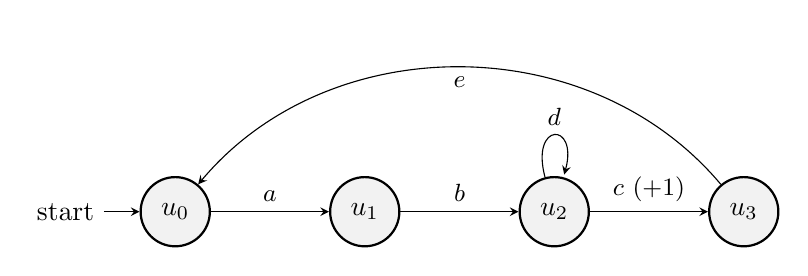
\begin{tikzpicture}[->, >=stealth, node distance=2.8cm, every state/.style={thick, fill=gray!10}]
\node[state, initial] (u0) {$u_0$};
\node[state, right=1.5cm of u0] (u1) {$u_1$};
\node[state, right=1.5cm of u1] (u2) {$u_2$};
\node[state, right=1.5cm of u2] (u3) {$u_3$};

\path
    (u0) edge node[above] {\small $a$} (u1)
    (u1) edge node[above] {\small $b$} (u2)
    (u2) edge node[above] {\small $c$ (+1)} (u3)
    (u2) edge[loop above] node[above] {\small $d$} (u2)
    (u3) edge[bend right=50] node[below] {\small $e$} (u0);
\end{tikzpicture}}
\end{center}

\subsubsection{Condition-Based Transitions}

\begin{center}
\resizebox{\columnwidth}{!}{%
\begin{tabular}{clll}
\toprule
\textbf{Lbl} & \textbf{Trans.} & \textbf{Condition} & \textbf{Description} \\
\midrule
$a$ & $u_0 \!\to\! u_1$ & \texttt{face\_up} $\land$ $\EBel{\text{money}\_p}$ & Sees money card \\
$b$ & $u_1 \!\to\! u_2$ & $\neg$\texttt{face\_up} $\land$ \texttt{cards\_mov.} & Shuffle begins \\
$c$ & $u_2 \!\to\! u_3$ & $\IBel{\text{money}\_p} \land \neg\text{money}\_p$ & \textbf{Deceived! (+1)} \\
$d$ & $u_2 \!\to\! u_2$ & \texttt{cards\_moving} & More shuffles \\
$e$ & $u_3 \!\to\! u_0$ & \texttt{show\_card} & Reset round \\
\bottomrule
\end{tabular}}
\end{center}

Transition $c$ is the epistemic core: the RM advances to $u_3$ and awards $+1.0$ only when the SAT solver confirms that the Observer holds a false belief about the money card's position.
Transition $e$ resets the RM to $u_0$ after a successful deception, allowing the dealer to reveal the cards (correcting the Observer's beliefs) and begin a new round.
The agent can accumulate $+1.0$ for each successful deception cycle within the episode's step budget, incentivising repeated deceptions.

\subsubsection{Reward Structure}

A reward of $+1.0$ is given on transition $c$ ($u_2 \to u_3$) when the Observer holds a false belief about the money card's position. All other transitions carry zero reward.
From $u_3$, transition $e$ loops back to $u_0$ for another round. The agent can perform multiple deception cycles per episode, accumulating $+1.0$ per cycle (analogous to the Chop Cup's lime loop between $u_T$ and $u_4$).

\subsection{Baseline Comparison}

We compare three methods adapted to the Three-Card Monte domain:
\begin{enumerate}
    \item \textbf{BEQRM}: Belief-Epistemic QRM with epistemic observations and RM-decomposed Q-tables.

    \item \textbf{HRL-RM}: Two-level option hierarchy with 3 subgoals (\emph{reveal}, \emph{hide}, \emph{shuffle}) plus epistemic observations and RM state.

    \item \textbf{DDQN}: Double Deep Q-Network (128-unit MLP) with the same epistemic observation (5 physical + 6 beliefs + RM index = 12 dimensions).
\end{enumerate}

All three methods were trained for 1000 episodes (\texttt{max\_steps}$=50$, $\gamma = 0.9$) and averaged over 5 random seeds. BEQRM and HRL-RM use tabular Q-learning ($\alpha = 0.05$, $\varepsilon = 0.1$); DDQN uses neural function approximation (Adam, $\text{lr}=10^{-3}$).

\subsubsection{Results}

\begin{figure}[ht]
\centering
\includegraphics[width=0.95\columnwidth]{three_card_results/comparison_success.pdf}
\caption{Three-Card Monte: success rate comparison (3-way, 5-seed average).}
\label{fig:tcm_comparison_success}
\end{figure}

\begin{figure}[ht]
\centering
\includegraphics[width=0.95\columnwidth]{three_card_results/comparison_reward.pdf}
\caption{Three-Card Monte: reward comparison (3-way, 5-seed average).}
\label{fig:tcm_comparison_reward}
\end{figure}

\begin{table}[ht]
\centering\small
\begin{tabular}{lccc}
\toprule
\textbf{Method} & \textbf{Success} & \textbf{Reward} & \textbf{Obs.\ Space} \\
\midrule
BEQRM & \textbf{100\%} & \textbf{6.8} & Epi.\ + RM (tabular) \\
HRL-RM & 100\% & 6.6 & Epi.\ + RM (tabular) \\
DDQN & 32.4\% & 0.3 & Epi.\ + RM (neural) \\
\bottomrule
\end{tabular}
\caption{Three-Card Monte: final performance after 1000 training episodes (5-seed average, $\alpha=0.05$).}
\label{tab:tcm_comparison}
\end{table}

\textbf{Key findings.}
\textbf{BEQRM outperforms HRL-RM.}
As in the Chop Cup, flat primitive actions (BEQRM) outperform the hierarchical variant (HRL-RM, 6.8 vs.\ 6.6 reward) because the Three-Card Monte's short cycle ($\sim$6 steps) does not benefit from temporal abstraction.
The option-selection overhead and SMDP discounting ($\gamma^k$) reduce the effective credit signal.

\textbf{DDQN struggles with the epistemic domain.}
DDQN achieves only 32.4\% success despite receiving the same observation as BEQRM.
The 12-dimensional state space is compact enough for exact tabular representation, and the discrete, logic-driven transitions are poorly suited for smooth function approximation.
The small state space means the neural network's capacity is wasted on generalisation that is not needed.

%%%%%%%%%%%%%%%%%%%%%%%%%%%%%%%%%%%%%%%%%%%%%%%%%%%%%%%%%%%%%%%%%%%%%%%%%%%%%%%%
\section{CONCLUSIONS}

We presented a self-contained Python implementation of epistemic reinforcement learning for the Chop Cup magic trick and the Three-Card Monte, with action effects faithfully mirroring their respective JSON specifications. The system demonstrates that SAT-based implicit belief reasoning can be effectively integrated into an RL loop, enabling agents to reason about and manipulate other agents' knowledge states. Belief transfer effects ($\triangle p := \triangle q$) are the critical mechanism enabling deception, and condition-based Reward Machines faithfully encode the temporal structure of the tricks. BEQRM exploits the RM structure to achieve 100\% deception success, outperforming hierarchical and neural baselines across both domains.

%%%%%%%%%%%%%%%%%%%%%%%%%%%%%%%%%%%%%%%%%%%%%%%%%%%%%%%%%%%%%%%%%%%%%%%%%%%%%%%%

\begin{thebibliography}{99}

\bibitem{engesser2025}
T.~Engesser, R.~Mattm\"{u}ller, and B.~Nebel,
``Epistemic Reinforcement Learning with Belief Bases,''
in {\it Proc.\ AAMAS 2025}, 2025.

\bibitem{icarte2018}
R.~T.~Icarte, T.~Q.~Klassen, R.~Valenzano, and S.~A.~McIlraith,
``Using Reward Machines for High-Level Task Specification and Decomposition in Reinforcement Learning,''
in {\it Proc.\ ICML 2018}, pp.~2107--2116, 2018.

\bibitem{bolander2011}
T.~Bolander and M.~B.~Andersen,
``Epistemic Planning for Single and Multi-Agent Systems,''
{\it J.\ Applied Non-Classical Logics}, vol.~21, no.~1, pp.~9--34, 2011.

\bibitem{rabinowitz2018}
N.~C.~Rabinowitz, F.~Perbet, H.~F.~Song, C.~Zhang, S.~M.~A.~Eslami, and M.~Botvinick,
``Machine Theory of Mind,''
in {\it Proc.\ ICML 2018}, pp.~4218--4227, 2018.

\bibitem{sutton1999}
R.~S.~Sutton, D.~Precup, and S.~Singh,
``Between MDPs and Semi-MDPs: A Framework for Temporal Abstraction in Reinforcement Learning,''
{\it Artificial Intelligence}, vol.~112, no.~1--2, pp.~181--211, 1999.

\bibitem{vanhasselt2016}
H.~van Hasselt, A.~Guez, and D.~Silver,
``Deep Reinforcement Learning with Double Q-Learning,''
in {\it Proc.\ AAAI 2016}, pp.~2094--2100, 2016.

\bibitem{ng1999}
A.~Y.~Ng, D.~Harada, and S.~Russell,
``Policy Invariance Under Reward Transformations: Theory and Application to Reward Shaping,''
in {\it Proc.\ ICML 1999}, pp.~278--287, 1999.

\bibitem{watkins1992}
C.~J.~C.~H.~Watkins and P.~Dayan,
``Q-Learning,''
{\it Machine Learning}, vol.~8, no.~3--4, pp.~279--292, 1992.

\bibitem{tsitsiklis1994}
J.~N.~Tsitsiklis,
``Asynchronous Stochastic Approximation and Q-Learning,''
{\it Machine Learning}, vol.~16, no.~3, pp.~185--202, 1994.

\bibitem{jaakkola1994}
T.~Jaakkola, M.~I.~Jordan, and S.~P.~Singh,
``On the Convergence of Stochastic Iterative Dynamic Programming Algorithms,''
{\it Neural Computation}, vol.~6, no.~6, pp.~1185--1201, 1994.

\bibitem{even-dar2003}
E.~Even-Dar and Y.~Mansour,
``Learning Rates for Q-Learning,''
{\it J.\ Machine Learning Research}, vol.~5, pp.~1--25, 2003.

\end{thebibliography}

\end{document}
